% Created 2023-03-16 Thu 14:05
% Intended LaTeX compiler: pdflatex
\documentclass[11pt]{article}
\usepackage[utf8]{inputenc}
\usepackage[T1]{fontenc}
\usepackage{graphicx}
\usepackage{longtable}
\usepackage{wrapfig}
\usepackage{rotating}
\usepackage[normalem]{ulem}
\usepackage{amsmath}
\usepackage{amssymb}
\usepackage{capt-of}
\usepackage{hyperref}
\author{3/c Christian Johnson}
\date{\today}
\title{DCCS Lab 4 Writeup}
\hypersetup{
 pdfauthor={3/c Christian Johnson},
 pdftitle={DCCS Lab 4 Writeup},
 pdfkeywords={},
 pdfsubject={},
 pdfcreator={Emacs 28.2 (Org mode 9.5.5)}, 
 pdflang={English}}
\begin{document}

\maketitle
\tableofcontents

\clearpage
\section{Abstract}
\label{sec:org594e886}
This lab expanded on basic circuit design, covering more advanced GUI concepts discussed in labs one and two. The user would input a hexadecimal character into the GUI app. This value is compared to two hardcoded values, and depending on which value it matches, will select different circuit functionality. The circuit switches between a voltmeter which varies based on a slider output from the GUI app, and a binary string output that varies based on a variable resistor. My Matlab code consisted mainly of the built-in Matlab conversions and Arduino write/read functions. These work together to format and then utilize various input and output values in order to properly interpret the information being sent to and from the Arduino. Since this particular lab involved both reading from and writing to the same set of pins, my code also relied upon an Arduino function that resets the current pin value – this ensures that at any given time the Arduino is sending data in the correct direction. Without these functions, the code would not function, and could damage the board itself. Overall, I was able to create a functioning board which effectively switched between functions and safely maanged the bidirectional flow of data. 

\section{Methodology}
\label{sec:org24687e2}
Lab 3 and Lab 4 were similar. Lab 3 consisted of a comparator which would select two different circuit functions based on user input to a MATLAB GUI application. These functions; a potentiometer and a set of toggle switches; both took physical input and wrote information to the Arduino board, which was then represented in the GUI. Lab 4 expanded on this structure, replacing the switches with a voltmeter that would represent a sequential series of voltage values based on user input to a slider in the GUI. This change was particularly significant, as it represented the shift from a unidirectional bus to a bidirectional bus. Circuit diagrams for both circuits are included in the attached appendices (Figures 2 and 5). These diagrams show the functional distinction between the unidirectional data transfer in Lab 3 and the bidirectional bus in lab four. In practice, a user would enter a value into the GUI, which would then be passed in binary from the Arduino into the comparator. If the input value matched either of the two hardcoded values, then the comparator would select the corresponding output. This output served to enable a flip flop, which was wired to support a different functionality (either the potentiometer, or the switches/voltmeter). In the case of Lab 3, the user would then interact with either the switches, or the potentiometer to generate an output, which would be passed back to the GUI. In Lab 4, the potentiometer functioned the same as in Lab 3, passing output back to the Arduino, but if the voltmeter was active, it took input from the GUI and registered it as a changing voltage value. 

\section{Results and Analysis}
\label{sec:orgf3f6db4}
Labs 3 and 4 utilized a variety of circuit elements to accomplish their respective objectives. These elements included various logic gates, flip flops, ADC’s, DAC’s, a potentiometer, switches, and a voltmeter. One of the components that initially confused me while I was constructing this circuit was the comparator. It took me some time to understand how the comparator was supposed to select each circuit function, and I was not able to get my circuit to properly work until I took the time to fully understand the comparator. Practically, the comparator acts as a simple switch. Internally however, it is slightly more complicated. It uses various logic gates to compare user input to pre-defined, hardwired inputs, and then outputs to a different pin depending on which of the two hardwired values is entered. These pins led to two different sets of flip flops, which function as data storage and transfer devices. They take a selection input from the comparator and general inputs from other elements before passing an output. They are only able to take and store inputs when the output-enable pin is given a logical low (as described in the Lab 3 Handout). This is relevant, because this is part of the tri-state structure that helps to protect our circuit and allows us to create a multifunction circuit. This tri-state device structure was integral to the circuit. Tri-state devices are circuit elements that have three states: On, Off, and Hi-Impedance. On and off are self-explanatory, but the Hi-Impedance state allows the element to be physically connected to the circuit while not drawing any current. This is important for multi-functional circuits since it allows the user to safely switch between several circuit functions without damaging the component elements. A properly designed circuit will utilize tri-state devices such that any element which could be damaged by an ongoing operation will be in the hi-impedance state, so that it is effectively “disconnected” from the active portions of the circuit. Theoretically, these devices would also allow us to connect more than two circuit functions (effectively expanding the bus). All we would need to do is connect the other elements to the bus, and wire them to the capacitor in such a way that they were in the correct state at the right time (i.e. use the tri-state devices to ensure that elements that are not active are either off, or hi-impedance depending on their functionality – although they should likely be in the hi-impedance state for safety). Since Lab 4 involved bi-directional data flow, we had to take steps to ensure that this data did not interfere with any information flowing the opposite direction. In order to do this, we utilized the tri-state devices to ensure that only devices that were in use were active at any given time, and then we added several lines of code to our button functions that formatted the Arduino to either receive or transmit information, depending on which circuit function was in use. 

\section{Conclusion}
\label{sec:orgd73ace5}
Over the course of this project, we explored different ways to integrate multiple functions into a single circuit. We created a bidirectional bus system which effectively transported data in two directions between analog and digital sources, and properly converted data formats. We created a GUI to interact with each circuit element and interpret data coming from those elements, and we practiced troubleshooting – debugging our code to properly interpret data and troubleshooting wiring errors in order to generate the expected circuit response. This project allowed us to gain the necessary skills to construct similar circuits on our own.

\clearpage
\section{Appendix}
\label{sec:orgd8b942e}

\subsection{Images}
\label{sec:org4c34073}

\begin{figure}[htbp]
\centering
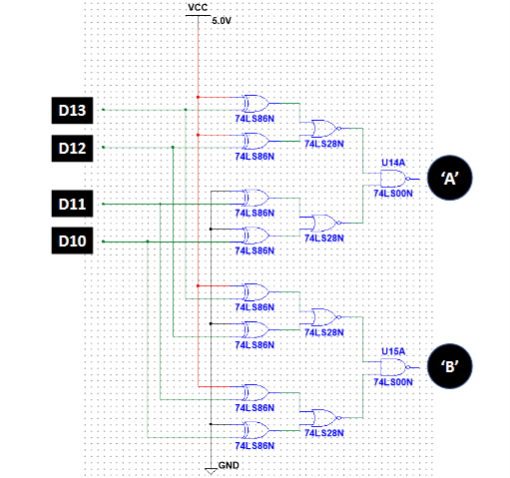
\includegraphics[width=.9\linewidth]{c:/Users/Christian/Documents/GitHub/OrgFiles/Class Notes/Files/Attachments/Lab3Diagram1.png}
\caption{Comparator Diagram Lab 3}
\end{figure}

\begin{figure}[htbp]
\centering
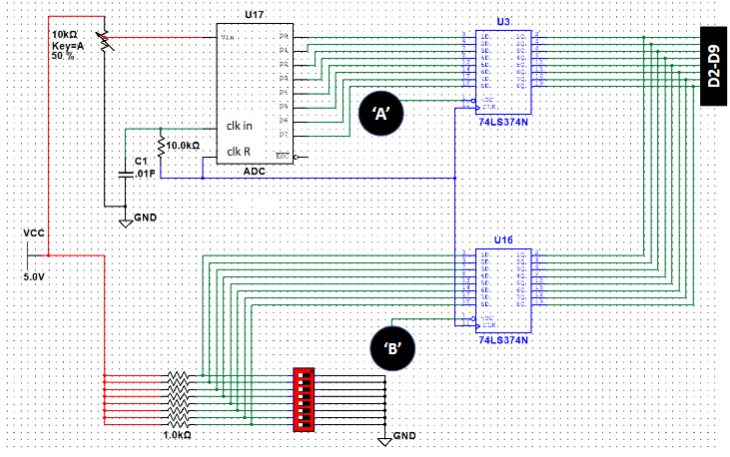
\includegraphics[width=.9\linewidth]{c:/Users/Christian/Documents/GitHub/OrgFiles/Class Notes/Files/Attachments/Lab3Diagram2.png}
\caption{Circuit Diagram Lab 3}
\end{figure}

\begin{figure}[htbp]
\centering
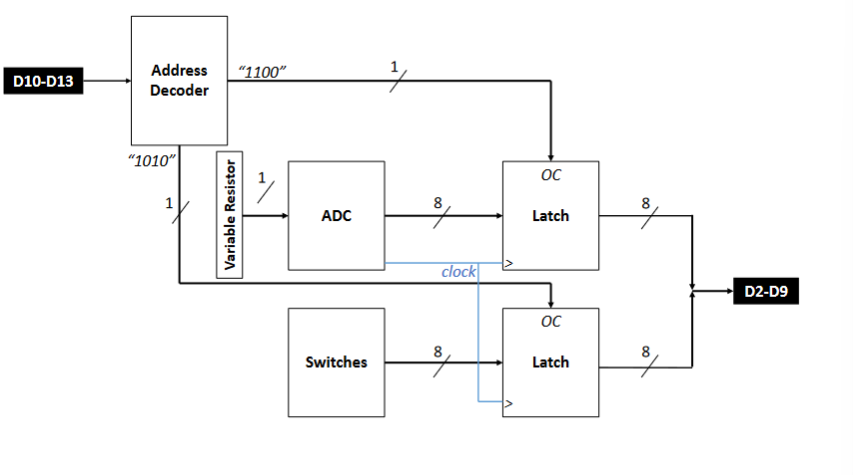
\includegraphics[width=.9\linewidth]{c:/Users/Christian/Documents/GitHub/OrgFiles/Class Notes/Files/Attachments/Lab3Diagram3.png}
\caption{Block Diagram Lab 3}
\end{figure}

\begin{figure}[htbp]
\centering
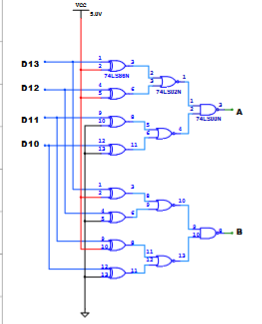
\includegraphics[width=.9\linewidth]{c:/Users/Christian/Documents/GitHub/OrgFiles/Class Notes/Files/Attachments/Lab4Diagram1.png}
\caption{Comparator Diagram Lab 4}
\end{figure}

\begin{figure}[htbp]
\centering
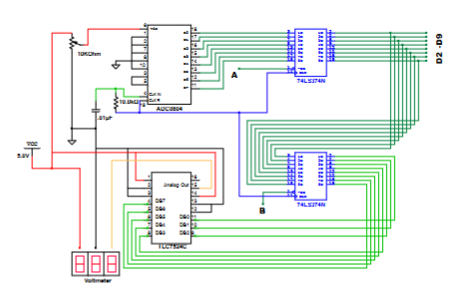
\includegraphics[width=.9\linewidth]{c:/Users/Christian/Documents/GitHub/OrgFiles/Class Notes/Files/Attachments/Lab4Diagram2.png}
\caption{Circuit Diagram Lab 4}
\end{figure}

\begin{figure}[htbp]
\centering
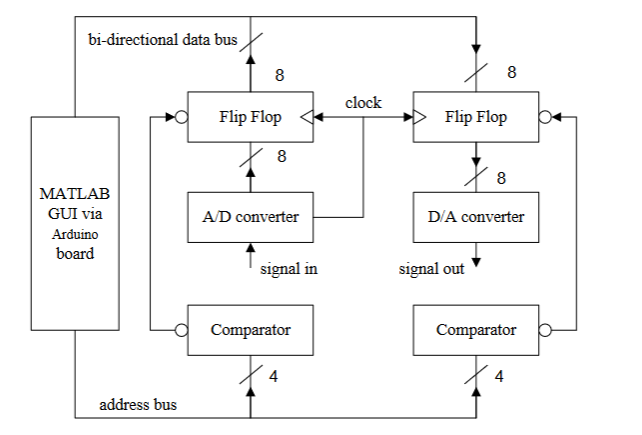
\includegraphics[width=.9\linewidth]{c:/Users/Christian/Documents/GitHub/OrgFiles/Class Notes/Files/Attachments/Lab4Diagram3.png}
\caption{Block Diagram Lab 4}
\end{figure}

\clearpage
\subsection{Code}
\label{sec:org71d03dd}

\begin{verbatim}
classdef ARDUINO_BI_Bus < matlab.apps.AppBase

    % Properties that correspond to app components
    properties (Access = public)
	UIFigure            matlab.ui.Figure
	Slider              matlab.ui.control.Slider
	Stop                matlab.ui.control.Button
	Start               matlab.ui.control.Button
	DataLabel           matlab.ui.control.Label
	ArduinoOut          matlab.ui.control.EditField
	BinaryField         matlab.ui.control.EditField
	HexField            matlab.ui.control.EditField
	CLRButton           matlab.ui.control.Button
	EnterButton         matlab.ui.control.Button
	HexadecimalInLabel  matlab.ui.control.Label
	BinaryOutLabel      matlab.ui.control.Label
	B0                  matlab.ui.control.Button
	B1                  matlab.ui.control.Button
	B2                  matlab.ui.control.Button
	B3                  matlab.ui.control.Button
	B4                  matlab.ui.control.Button
	B5                  matlab.ui.control.Button
	B6                  matlab.ui.control.Button
	B7                  matlab.ui.control.Button
	B8                  matlab.ui.control.Button
	B9                  matlab.ui.control.Button
	BA                  matlab.ui.control.Button
	BB                  matlab.ui.control.Button
	BC                  matlab.ui.control.Button
	BD                  matlab.ui.control.Button
	BE                  matlab.ui.control.Button
	BF                  matlab.ui.control.Button
    end


    properties (Access = private)
	BINValue % Binary Field Value
	HEXValue % Hexadecimal Field Value
	H2BConv % Buffer for conversion math
	My_Board %Board Variable


	Output % Outputs to the Board
	Input % Stores Board Input
	loopclock % Loop Control for clock

	Data % Description
	loopvolt % Loop Control for voltmeter
	SliderConvert1 % Convert Slider Dec to Bin
	SliderConvert2 % Change to string
    end

    methods (Access = private)

	function results = DIO(app, address)%defines callback for function

	    if isempty(app.My_Board)
		app.My_Board=arduino(); %adds boar dif not found
	    end 

	    bit0 = str2num(address(4)); %sets position for bit0
	    bit1 = str2num(address(3));%sets position for bit1
	    bit2 = str2num(address(2));%sets position for bit2
	    bit3 = str2num(address(1));%sets position for bit3

	    writeDigitalPin(app.My_Board, 'D10', bit0);%outputs to pin
	    writeDigitalPin(app.My_Board, 'D11', bit1);%outputs to pin
	    writeDigitalPin(app.My_Board, 'D12', bit2);%outputs to pin
	    writeDigitalPin(app.My_Board, 'D13', bit3);%outputs to pin

	end
    end


    % Callbacks that handle component events
    methods (Access = private)

	% Code that executes after component creation
	function startupFcn(app)
	    app.BINValue=""; %initializes values
	    app.HEXValue="";
	    if isempty(app.My_Board)
		app.My_Board=arduino(); %adds boar dif not found
	    end 
	end

	% Button pushed function: B0
	function B0ButtonPushed(app, event)
	    app.HEXValue = "0"; %Sets buffer variable, then sets display
	    app.HexField.Value = (app.HEXValue);
	end

	% Button pushed function: B1
	function B1ButtonPushed(app, event)
	    app.HEXValue = "1";%Sets buffer variable, then sets display
	    app.HexField.Value = (app.HEXValue);
	end

	% Button pushed function: B2
	function B2ButtonPushed(app, event)
	   app.HEXValue = "2";%Sets buffer variable, then sets display
	    app.HexField.Value = (app.HEXValue); 
	end

	% Button pushed function: B3
	function B3ButtonPushed(app, event)
	    app.HEXValue = "3";%Sets buffer variable, then sets display
	    app.HexField.Value = (app.HEXValue);
	    app.loopclock=true;
	    configurePin(app.My_Board, 'D2', 'Unset');
	    configurePin(app.My_Board, 'D3', 'Unset');
	    configurePin(app.My_Board, 'D4', 'Unset');
	    configurePin(app.My_Board, 'D5', 'Unset');
	    configurePin(app.My_Board, 'D6', 'Unset');
	    configurePin(app.My_Board, 'D7', 'Unset');
	    configurePin(app.My_Board, 'D8', 'Unset');
	    configurePin(app.My_Board, 'D9', 'Unset');

	end

	% Button pushed function: B4
	function B4ButtonPushed(app, event)
	    app.HEXValue = "4";%Sets buffer variable, then sets display
	    app.HexField.Value = (app.HEXValue);
	end

	% Button pushed function: B5
	function B5ButtonPushed(app, event)
	    app.HEXValue = "5";%Sets buffer variable, then sets display
	    app.HexField.Value = (app.HEXValue);
	    app.loopvolt=true;
	    configurePin(app.My_Board, 'D2', 'Unset');
	    configurePin(app.My_Board, 'D3', 'Unset');
	    configurePin(app.My_Board, 'D4', 'Unset');
	    configurePin(app.My_Board, 'D5', 'Unset');
	    configurePin(app.My_Board, 'D6', 'Unset');
	    configurePin(app.My_Board, 'D7', 'Unset');
	    configurePin(app.My_Board, 'D8', 'Unset');
	    configurePin(app.My_Board, 'D9', 'Unset');

	end

	% Button pushed function: B6
	function B6ButtonPushed(app, event)
	    app.HEXValue = "6";%Sets buffer variable, then sets display
	    app.HexField.Value = (app.HEXValue);
	end

	% Button pushed function: B7
	function B7ButtonPushed(app, event)
	    app.HEXValue = "7";%Sets buffer variable, then sets display
	    app.HexField.Value = (app.HEXValue);
	end

	% Button pushed function: B8
	function B8ButtonPushed(app, event)
	    app.HEXValue = "8";%Sets buffer variable, then sets display
	    app.HexField.Value = (app.HEXValue);
	end

	% Button pushed function: B9
	function B9ButtonPushed(app, event)
	    app.HEXValue = "9";%Sets buffer variable, then sets display
	    app.HexField.Value = (app.HEXValue);
	end

	% Button pushed function: BA
	function BAButtonPushed(app, event)
	    app.HEXValue = "A";%Sets buffer variable, then sets display
	    app.HexField.Value = (app.HEXValue);
	end

	% Button pushed function: BB
	function BBButtonPushed(app, event)
	    app.HEXValue = "B";%Sets buffer variable, then sets display
	    app.HexField.Value = (app.HEXValue);
	end

	% Button pushed function: BC
	function BCButtonPushed(app, event)
	    app.HEXValue = "C";%Sets buffer variable, then sets display
	    app.HexField.Value = (app.HEXValue);
	end

	% Button pushed function: BD
	function BDButtonPushed(app, event)
	    app.HEXValue = "D";%Sets buffer variable, then sets display
	    app.HexField.Value = (app.HEXValue);
	end

	% Button pushed function: BE
	function BEButtonPushed(app, event)
	    app.HEXValue = "E";%Sets buffer variable, then sets display
	    app.HexField.Value = (app.HEXValue);
	end

	% Button pushed function: BF
	function BFButtonPushed(app, event)
	    app.HEXValue = "F";%Sets buffer variable, then sets display
	    app.HexField.Value = (app.HEXValue);
	end

	% Button pushed function: CLRButton
	function CLRButtonPushed(app, event)
	    app.HEXValue = "0";%Sets buffer variable, then sets display
	    app.BINValue = "0";%Zeroes clear for new entry
	    app.BinaryField.Value = "0000";
	    app.HexField.Value = "0000";
	end

	% Button pushed function: EnterButton
	function EnterButtonPushed(app, event)
	    hexStr = app.HEXValue;%sets buffer variable for conversion
	    app.H2BConv = dec2bin(hex2dec(hexStr),4);%converts
	    app.BINValue = app.H2BConv;%4 in conversion is for length
	    app.BinaryField.Value = app.BINValue;%sets display 
	    %DIO(app, app.BINValue);%runs function for arduino with args




	end

	% Button pushed function: Start
	function StartButtonPushed(app, event)
	    %app.loopclock = true;
	    app.Data = '00000000';

	    configurePin(app.My_Board, 'D2', 'Unset');
	    configurePin(app.My_Board, 'D3', 'Unset');
	    configurePin(app.My_Board, 'D4', 'Unset');
	    configurePin(app.My_Board, 'D5', 'Unset');
	    configurePin(app.My_Board, 'D6', 'Unset');
	    configurePin(app.My_Board, 'D7', 'Unset');
	    configurePin(app.My_Board, 'D8', 'Unset');
	    configurePin(app.My_Board, 'D9', 'Unset');

	    app.Output = app.BINValue;
	    DIO(app, app.Output);
	    while( app.loopclock ) % runs until stop
		app.Data(1) = num2str(readDigitalPin(app.My_Board,'D2'));
		app.Data(2) = num2str(readDigitalPin(app.My_Board,'D3'));
		app.Data(3) = num2str(readDigitalPin(app.My_Board,'D4'));
		app.Data(4) = num2str(readDigitalPin(app.My_Board,'D5'));
		app.Data(5) = num2str(readDigitalPin(app.My_Board,'D6'));
		app.Data(6) = num2str(readDigitalPin(app.My_Board,'D7'));
		app.Data(7) = num2str(readDigitalPin(app.My_Board,'D8'));
		app.Data(8) = num2str(readDigitalPin(app.My_Board,'D9'));

		app.ArduinoOut.Value = app.Data;
	    end

	    while( app.loopvolt ) %runs until stop
		app.SliderConvert1 = dec2bin((app.Slider.Value),8);

		writeDigitalPin(app.My_Board, 'D9', str2num(app.SliderConvert1(8)));
		writeDigitalPin(app.My_Board, 'D8', str2num(app.SliderConvert1(7)));
		writeDigitalPin(app.My_Board, 'D,7', str2num(app.SliderConvert1(6)));
		writeDigitalPin(app.My_Board, 'D6', str2num(app.SliderConvert1(5)));
		writeDigitalPin(app.My_Board, 'D5', str2num(app.SliderConvert1(4)));
		writeDigitalPin(app.My_Board, 'D4', str2num(app.SliderConvert1(3)));
		writeDigitalPin(app.My_Board, 'D3', str2num(app.SliderConvert1(2)));
		writeDigitalPin(app.My_Board, 'D2', str2num(app.SliderConvert1(1)));


		app.ArduinoOut.Value = app.SliderConvert1;

	    end


	end

	% Button pushed function: Stop
	function StopButtonPushed(app, event)
	    app.loopclock = false;
	    app.loopvolt = false;
	end
    end

    % Component initialization
    methods (Access = private)

	% Create UIFigure and components
	function createComponents(app)

	    % Create UIFigure and hide until all components are created
	    app.UIFigure = uifigure('Visible', 'off');
	    app.UIFigure.Color = [0.8 0.8 0.8];
	    app.UIFigure.Position = [80 1 255 513];
	    app.UIFigure.Name = 'MATLAB App';

	    % Create BF
	    app.BF = uibutton(app.UIFigure, 'push');
	    app.BF.ButtonPushedFcn = createCallbackFcn(app, @BFButtonPushed, true);
	    app.BF.Position = [192 75 41 40];
	    app.BF.Text = 'F';

	    % Create BE
	    app.BE = uibutton(app.UIFigure, 'push');
	    app.BE.ButtonPushedFcn = createCallbackFcn(app, @BEButtonPushed, true);
	    app.BE.Position = [135 75 41 40];
	    app.BE.Text = 'E';

	    % Create BD
	    app.BD = uibutton(app.UIFigure, 'push');
	    app.BD.ButtonPushedFcn = createCallbackFcn(app, @BDButtonPushed, true);
	    app.BD.Position = [82 75 41 40];
	    app.BD.Text = 'D';

	    % Create BC
	    app.BC = uibutton(app.UIFigure, 'push');
	    app.BC.ButtonPushedFcn = createCallbackFcn(app, @BCButtonPushed, true);
	    app.BC.Position = [30 75 41 40];
	    app.BC.Text = {'C'; ''};

	    % Create BB
	    app.BB = uibutton(app.UIFigure, 'push');
	    app.BB.ButtonPushedFcn = createCallbackFcn(app, @BBButtonPushed, true);
	    app.BB.Position = [192 129 41 40];
	    app.BB.Text = 'B';

	    % Create BA
	    app.BA = uibutton(app.UIFigure, 'push');
	    app.BA.ButtonPushedFcn = createCallbackFcn(app, @BAButtonPushed, true);
	    app.BA.Position = [135 129 41 40];
	    app.BA.Text = 'A';

	    % Create B9
	    app.B9 = uibutton(app.UIFigure, 'push');
	    app.B9.ButtonPushedFcn = createCallbackFcn(app, @B9ButtonPushed, true);
	    app.B9.Position = [82 129 41 40];
	    app.B9.Text = {'9'; ''};

	    % Create B8
	    app.B8 = uibutton(app.UIFigure, 'push');
	    app.B8.ButtonPushedFcn = createCallbackFcn(app, @B8ButtonPushed, true);
	    app.B8.Position = [30 129 41 40];
	    app.B8.Text = {'8'; ''};

	    % Create B7
	    app.B7 = uibutton(app.UIFigure, 'push');
	    app.B7.ButtonPushedFcn = createCallbackFcn(app, @B7ButtonPushed, true);
	    app.B7.Position = [192 183 41 40];
	    app.B7.Text = {'7'; ''};

	    % Create B6
	    app.B6 = uibutton(app.UIFigure, 'push');
	    app.B6.ButtonPushedFcn = createCallbackFcn(app, @B6ButtonPushed, true);
	    app.B6.Position = [135 183 41 40];
	    app.B6.Text = {'6'; ''};

	    % Create B5
	    app.B5 = uibutton(app.UIFigure, 'push');
	    app.B5.ButtonPushedFcn = createCallbackFcn(app, @B5ButtonPushed, true);
	    app.B5.Position = [82 183 41 40];
	    app.B5.Text = {'5'; ''};

	    % Create B4
	    app.B4 = uibutton(app.UIFigure, 'push');
	    app.B4.ButtonPushedFcn = createCallbackFcn(app, @B4ButtonPushed, true);
	    app.B4.Position = [31 183 41 40];
	    app.B4.Text = {'4'; ''};

	    % Create B3
	    app.B3 = uibutton(app.UIFigure, 'push');
	    app.B3.ButtonPushedFcn = createCallbackFcn(app, @B3ButtonPushed, true);
	    app.B3.Position = [192 235 41 40];
	    app.B3.Text = {'3'; ''};

	    % Create B2
	    app.B2 = uibutton(app.UIFigure, 'push');
	    app.B2.ButtonPushedFcn = createCallbackFcn(app, @B2ButtonPushed, true);
	    app.B2.Position = [135 235 41 40];
	    app.B2.Text = {'2'; ''};

	    % Create B1
	    app.B1 = uibutton(app.UIFigure, 'push');
	    app.B1.ButtonPushedFcn = createCallbackFcn(app, @B1ButtonPushed, true);
	    app.B1.Position = [82 235 41 40];
	    app.B1.Text = '1';

	    % Create B0
	    app.B0 = uibutton(app.UIFigure, 'push');
	    app.B0.ButtonPushedFcn = createCallbackFcn(app, @B0ButtonPushed, true);
	    app.B0.Position = [30 235 41 40];
	    app.B0.Text = '0';

	    % Create BinaryOutLabel
	    app.BinaryOutLabel = uilabel(app.UIFigure);
	    app.BinaryOutLabel.HorizontalAlignment = 'center';
	    app.BinaryOutLabel.Position = [28 363 203 24];
	    app.BinaryOutLabel.Text = 'Binary Out';

	    % Create HexadecimalInLabel
	    app.HexadecimalInLabel = uilabel(app.UIFigure);
	    app.HexadecimalInLabel.HorizontalAlignment = 'center';
	    app.HexadecimalInLabel.Position = [29 316 202 23];
	    app.HexadecimalInLabel.Text = {'Hexadecimal In'; ''};

	    % Create EnterButton
	    app.EnterButton = uibutton(app.UIFigure, 'push');
	    app.EnterButton.ButtonPushedFcn = createCallbackFcn(app, @EnterButtonPushed, true);
	    app.EnterButton.Position = [135 20 45 40];
	    app.EnterButton.Text = {'Enter'; ''};

	    % Create CLRButton
	    app.CLRButton = uibutton(app.UIFigure, 'push');
	    app.CLRButton.ButtonPushedFcn = createCallbackFcn(app, @CLRButtonPushed, true);
	    app.CLRButton.Position = [193 20 40 40];
	    app.CLRButton.Text = {'CLR'; ''};

	    % Create HexField
	    app.HexField = uieditfield(app.UIFigure, 'text');
	    app.HexField.HorizontalAlignment = 'right';
	    app.HexField.Position = [29 291 202 25];

	    % Create BinaryField
	    app.BinaryField = uieditfield(app.UIFigure, 'text');
	    app.BinaryField.HorizontalAlignment = 'right';
	    app.BinaryField.Position = [31 340 200 24];

	    % Create ArduinoOut
	    app.ArduinoOut = uieditfield(app.UIFigure, 'text');
	    app.ArduinoOut.HorizontalAlignment = 'right';
	    app.ArduinoOut.Position = [29 452 200 24];

	    % Create DataLabel
	    app.DataLabel = uilabel(app.UIFigure);
	    app.DataLabel.Position = [114 473 31 22];
	    app.DataLabel.Text = 'Data';

	    % Create Start
	    app.Start = uibutton(app.UIFigure, 'push');
	    app.Start.ButtonPushedFcn = createCallbackFcn(app, @StartButtonPushed, true);
	    app.Start.Position = [30 20 41 40];
	    app.Start.Text = {'Start'; ''};

	    % Create Stop
	    app.Stop = uibutton(app.UIFigure, 'push');
	    app.Stop.ButtonPushedFcn = createCallbackFcn(app, @StopButtonPushed, true);
	    app.Stop.Position = [82 20 41 40];
	    app.Stop.Text = {'Stop'; ''};

	    % Create Slider
	    app.Slider = uislider(app.UIFigure);
	    app.Slider.Limits = [0 255];
	    app.Slider.Position = [43 428 174 3];

	    % Show the figure after all components are created
	    app.UIFigure.Visible = 'on';
	end
    end

    % App creation and deletion
    methods (Access = public)

	% Construct app
	function app = ARDUINO_BI_Bus

	    % Create UIFigure and components
	    createComponents(app)

	    % Register the app with App Designer
	    registerApp(app, app.UIFigure)

	    % Execute the startup function
	    runStartupFcn(app, @startupFcn)

	    if nargout == 0
		clear app
	    end
	end

	% Code that executes before app deletion
	function delete(app)

	    % Delete UIFigure when app is deleted
	    delete(app.UIFigure)
	end
    end
end
\end{verbatim}
\end{document}